\documentclass[%
bachelor,    % тип документа
natbib,      % использовать пакет natbib для "сжатия" цитирований
subf,        % использовать пакет subcaption для вложенной нумерации рисунков
href,        % использовать пакет hyperref для создания гиперссылок
colorlinks,  % цветные гиперссылки
%fixint,     % включить прямые знаки интегралов
]{disser}

\usepackage[
a4paper, mag=1000,
left=2.5cm, right=1cm, top=2cm, bottom=2cm, headsep=0.7cm, footskip=1cm
]{geometry}

\usepackage[intlimits]{amsmath}
\usepackage{amssymb,amsfonts}

\usepackage[T2A]{fontenc}
\usepackage[utf8]{inputenc}
\usepackage[english,russian]{babel}
\ifpdf\usepackage{epstopdf}\fi
\usepackage[autostyle]{csquotes}

% Шрифт Times в тексте как основной
%\usepackage{tempora}
\usepackage{setspace}
% альтернативный пакет из дистрибутива TeX Live
%\usepackage{cyrtimes}

% Шрифт Times в формулах как основной
%\usepackage[varg,cmbraces,cmintegrals]{newtxmath}
% альтернативный пакет
%\usepackage[subscriptcorrection,nofontinfo]{mtpro2}

% Плавающие рисунки "в оборку".
\usepackage{wrapfig}

% Номера страниц снизу и по центру
%\pagestyle{footcenter}
%\chapterpagestyle{footcenter}

% Точка с запятой в качестве разделителя между номерами цитирований
%\setcitestyle{semicolon}

% Использовать полужирное начертание для векторов
\let\vec=\mathbf
%______________________________-
\usepackage{lipsum}

%\usepackage{titlesec}
%\usepackage{spacing}
%\titleformat{\section}[block]{\color{blue}\Large\bfseries\filcenter}{}{1em}{}
% Номера страниц снизу и по центру
\pagestyle{footcenter}
\chapterpagestyle{footcenter}

% Точка с запятой в качестве разделителя между номерами цитирований
%\setcitestyle{semicolon}



% Переопределение стандартных заголовков
%\def\contentsname{Содержание}
%\def\conclusionname{Выводы}
%\def\bibname{Литература}

\usepackage{geometry} % пакет для установки полей
\geometry{top=1.5cm} % отступ сверху
\geometry{bottom=2cm} % отступ снизу
\geometry{left=3cm} % отступ справа
\geometry{right=1.5cm} % отступ слева
\newcommand{\sectionbreak}{\clearpage}
\newcommand*{\No}{\textnumero}
\renewcommand{\Re}{\mathrm{Re}}
\renewcommand{\Im}{\mathrm{Im}}

\newcommand{\const}{\mathrm{const}}
\newcommand{\arccosh}{\mathrm{arccosh}}

\newcommand{\vF}{\mathbf{F}}
\newcommand{\ve}{\mathbf{e}}
\newcommand{\vk}{\mathbf{k}}
\newcommand{\vq}{\mathbf{q}}
\newcommand{\vp}{\mathbf{p}}
\newcommand{\va}{\mathbf{a}}
\newcommand{\vP}{\mathbf{P}}
\newcommand{\vK}{\mathbf{K}}
\newcommand{\vQ}{\mathbf{Q}}
\newcommand{\vA}{\mathbf{A}}
\newcommand{\vr}{\mathbf{r}}
\newcommand{\vR}{\mathbf{R}}

\newcommand{\vRR}{\boldsymbol{\mathcal{R}}}
\newcommand{\veps}{\boldsymbol{\varepsilon}}

\newcommand{\cA}{\mathcal{A}}
\newcommand{\cR}{\mathcal{R}}
\newcommand{\cM}{\mathcal{M}}
\newcommand{\cE}{\mathcal{E}}
\newcommand{\cJ}{\mathcal{J}}
\newcommand{\cT}{\mathcal{T}}
\newcommand{\cD}{\mathcal{D}}


%______________________________-
% Включать подсекции в оглавление
\setcounter{tocdepth}{2}

\graphicspath{{fig/}}

\begin{document}
\section*{\centering Введение}
\addcontentsline{toc}{section}{Введение}

Вопрос о том, из чего сделан материальный мир и откуда все это произошло, интересовал людей со времен античности. Левкипп (около 430 г. до н.э.) и Демокрит
(около 420 г. до н.э.) первыми предложили атомную теорию, в которой вся материя состоит из
неделимых частиц. В средние века, различные исследователи, известные как алхимики, добились прогресса
в разработке экспериментальных методов исследования составляющих компонентов вещества. Однако,
их исследования в основном состояли из тщетных попыток превратить обычные металлы
(например, свинца) в благородные металлы (такие как золото), и не было достигнуто никакого прогресса в
развитии теории о том, как может произойти такое преобразование. Только в конце 20-го века современные алхимики, обычно
известные как ядерные физики, добились успеха в превращении висмута в золото
(в небольших количествах и по коммерчески неосуществимым расходам). Дорога, ведущая к этому знаменательному достижению, включала работы химиков (Бойл, 1661, де Лавуазье, 1789), современную атомной теории (Dalton, 1808, Avogadro, 1811, Thomson, 1897) и достижения в ядерной физике (Резерфорд, 1911; Чадвик, 1932; Ферми, 1934; Юкава, 1935), которые обеспечили нам хорошее понимание строительных блоков, из которых состоит материя.

Хорошее понимание того, что составляет материю, является необходимым первым шагом в развитии теорию о том, как эта материя была создана.  Alpher et al. (1948) выдвинул теорию, что все элементы были синтезированы во время Большого взрыва. Однако, когда более точнее сечение захвата нейтронов для ядер малой массы (A < 20) стало доступным, также стало ясно, что нуклеосинтез во время ранней расширяющейся вселенной не способен преодолеть A = 8 (например, Alpher and Herman, 1950; Shaviv, 2012). Это легло в основу работы Burbidge et al. (1957), который предложил, что лишь самые легкие элементы (в основном водород и гелий) возникли во время Большого взрыва, а более тяжелые элементы синтезируются в звездах. Хотя эта теория со временем была уточнена, оригинальная идея Бербиджа и др. (1957) выдержал испытание временем. Таково нынешнее понимание того, что различные ядерные процессы действительно ответственны за синтез всех элементов, более тяжелых, чем водород и гелий.

В данной работе я исследую процесс захвата быстрых нейтронов (r-процесс), который является одним из ядерных процессов, предположенных Burbidge et al. (1957) в результате которого возникают элементы тяжелее железа. Мое внимание сосредоточено на вычислении нуклеосинтеза r-процесса при слияним звезд при помощи нового инструмента для расчета ядерных реакций, SkyNey, который я разработал. В оставшейся части этого введения я кратко опишу текущее представление о происхождении элементов, сущность r-процесса, условия его возникновения и ожидаемые наблюдательные сигнатуры. В главе II я представляю физику, которая реализована в SkyNet для эволюции тысяч видов ядер под влиянием десятков тысяч ядерных реакций Я использую SkyNet в главе III, чтобы систематически исследовать r-процесс и его возможные оптические аналоги для различные параметров. В главе IV обсуждается нуклеосинтез r-процесса при слияниях черных дыр и нейтронных звезд (BHNS), а в главе V я рассматриваю rprocess
в оттоке диска (in the disk outflow following) после слияния нейтронных звезд. В главе VI я кратко подведу итог другой работы, которую я проделал во время моей докторской диссертации, которая не является непосредственно частью этой работы. Наконец, я предоставляю резюме и дальнейшие перспективы в главе VII.

\subsection{Распространенность в солнечной системе}
Стоит проверить теории и модели, которые предсказывают как создаются элементы и в каких отношениях, подробный перечень этих элементов и их относительная распространенность в данном участки вселенной. Крайне сложно получить образцы материи из мест, отличных от земной коры. Миссии Аполлона и Луны принесли образцы с луны, а позже такие космические аппараты, как Звездная пыль, Бытие и Hayabusa успешно доставили образцы из близлежащих астероидов и космической пыли на Землю. Однако подавляющее большинство внеземных материалов, доступных для химических анализов происходит от метеоритов, которые падают на поверхность Земли. Поэтому, чтобы определить состав звезд и других астрофизических объектов, мы ограничимся изучением линиями поглощения и излучения, формирующими эти объекты, а также распространенность элементарных частиц (например, Shaviv, 2012). Линии поглощения в солнечном спектре были впервые обнаружены в начале XIX век (Wollaston, 1802; Fraunhofer, 1817). Тем не менее, применение им нашли только 100 лет спустя, после развития квантовой механики, которая утверждает, что линии поглощения могут использоваться для количественного определения распространенности различных элементов на солнце. Пионерская работа была проведена Пейном (1925) в ее основной научной диссертации и Расселом (1934). Важная работа Суссе и Юри (1956) была одной из первых принимающих во внимание изотопные измерения распространенности из метеоритов. С этого момента был достигнут большой прогресс в измерении распространенности элементов и изотопов в нашей солнечной системе (например, Cameron, 1973; Anders and Grevesse, 1989; Grevesse and Sauval, 1998; Lodders, 2003).

\begin{figure}[h]
	\center{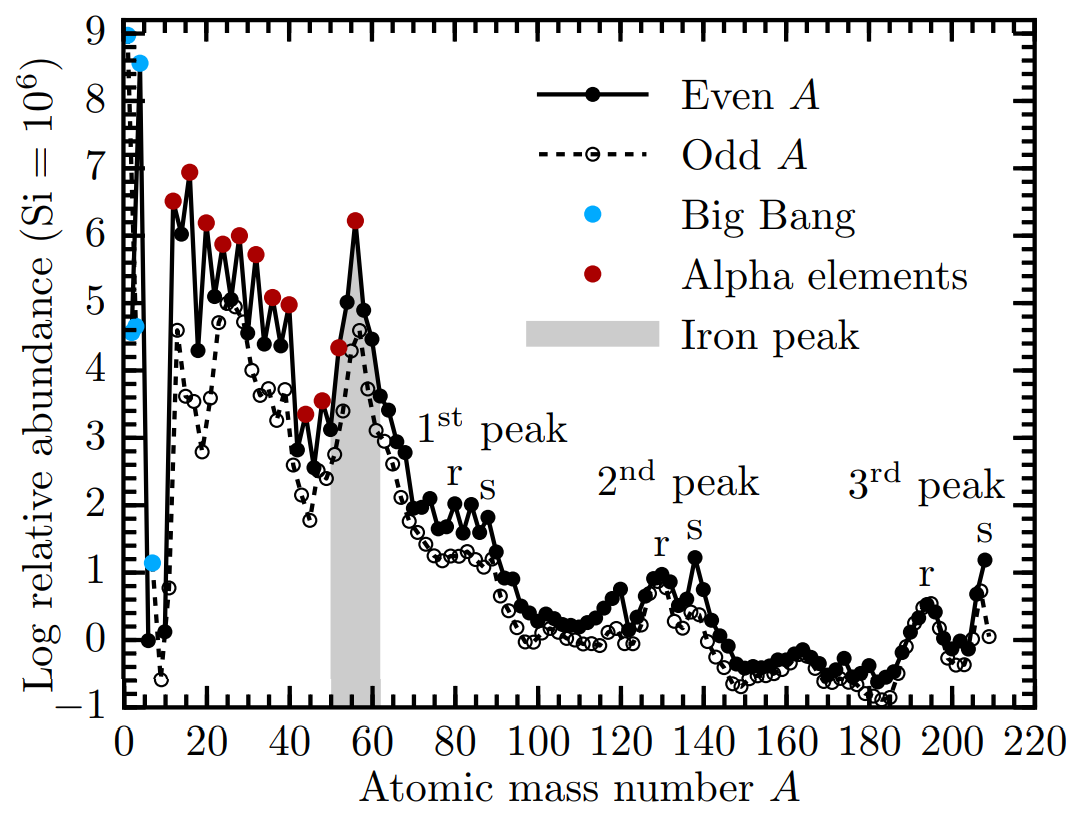
\includegraphics[width=0.7\linewidth]{1}}
	\caption{Наблюдаемая распространенность в нашей солнечной системе в зависимости от массового числа А. Самые легкие элементы были созданы в «Большом взрыве». Слияние в звездах преимущественно создает альфа-элементы. Пик железа выполнен в коллапсе ядра и типе Ia сверхновых. Элементы за железным пиком синтезируются медленными (s) и быстрыми (r) процессами захвата нейтронов. Эти процессы производят три пары пиков (см. раздел 1.3). Данные о изобилии от Lodders (2003).}
	\label{ris:1}
\end{figure}

На рис. \ref{ris:1} показаны наблюдаемые распространенности в нашей солнечной системе в зависимости от массового числа А (данные от Lodders 2003). Нуклиды с четным массовым числом как правило более многочисленными, чем нуклиды с нечетным массовым числом, поскольку даже массовые нуклиды более связаны. (!!!!!!even mass nuclides are more bound) Из-за спинового спаривания нуклонов нуклид с четным число нейтронов и протонов (следовательно, четное A) является более связанным, чем нуклид с нечетным числом нейтронов или протонов (следовательно, нечетное А, см., например, Weizsäcker, 1935; Майерс и Свитецки, 1966; Möller et al., 1995). Нуклиды с нечетное число и нейтронов и протонов (отсюда и четное A), имеют еще более слабую связь поскольку ни все нейтроны, ни все протоны не могут быть спин-парными. Поэтому неудивительно, что существует только несколько нечетных-нечетных нуклидов, которые являются стабильными или долгоживущими: 2H, 6Li, 10B и 14N стабильны, а 40K, 50V, 138La и 176Lu являются только нечетные-нечетные нуклиды с периодом полураспада не менее 1 Гр(!!!!!Gyr). Существует ряд различных процессов нуклеосинтеза, которые доминируют в различных диапазонах масс. Очень легкие нуклиды (A <8) были получены сразу после Большого взрыва. Некоторые $^4He$, а также большинство нуклидов в диапазоне 12 $<=$ A $<=$ 56 являются результатом гидростатического ядерного горения в звездах, значительная часть пика железа (50 .A .62) производится материалом, поступающим в (!!!!!nuclear statistical equilibrium) ядерную статистическую (NSE), а затем охлаждающимся (например, во время сверхновой звезды Ia или взрывчатое сильное сжигание в ядрах с коллапсом сверхновых (explosive silicon burning in core-collapse supernovae) (CCSNe)) и, наконец, почти все нуклиды, более тяжелые, чем железо, образуются путем захвата нейтронов на более легкие семенные ядра (!!!!!onto lighter seed nuclei) (например, Burbidge et al., 1957). Мы рассмотрим эти процессы далее.

\subsection{Нуклеосинтез Большого Взрыва}
\begin{figure}[h]
	\center{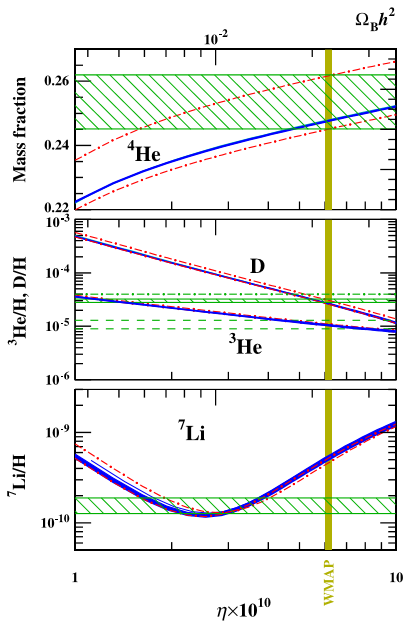
\includegraphics[width=0.7\linewidth]{2}}
	\caption{Вычисленная распространенность 4He, D, 3He и 7Li (синие линии) в зависимости от отношения барион-фотон $\eta$. Зеленые области - наблюдаемые концентрации, а желтая вертикальная полоса - наблюдаемое значение $\eta$. Вычисленные количества 4He, D и 3He согласуются с наблюдениями, но прогнозируется избыток 7Li в 4-5 $\sigma$. Это известная «литиевая проблема». Рисунок 1 из Cocetal. (2013)}
	\label{ris:2}
\end{figure}
Нуклеосинтез Большого Взрыва (BBN) создал в основном водород (~ 75$\%$ по массе) и гелий (~ 25$\%$ по массе) в промежутке от первых десяти секунд до минут после Большого взрыва, а также некоторое количества (!!!!trace - следовое) дейтерия, 3He и 7Li (см. Tytler et al., 2000 и ссылки в нем). 13,8 Gyr позже химический состав Вселенной оставался около 75$\%$ H и 25$\%$ He, потому что создание более тяжелых элементов требует экстремальных физических условий. Интересно, что BBN является проблемой для моделирования, потому что он включает лишь несколько нуклидов, в настоящее время существуют большие расхождения между результатами моделирование BBN и наблюдениями. Прогнозируемый дейтерий и распространенность 4He хорошо согласуется с наблюдениями, но модели BBN предсказывают большую распространенность 7Li на 4-5 $\sigma$ по сравнению с наблюдениями, см. рис. \ref{ris:2}, которая изображена на рисунке 1 от Coc et al. (2013). Это расхождение не до конца понятно и называется «литиевой проблемой». Предлагаемые причины этого включают систематические ошибки в наблюдениях численности 7Li, неизвестные или плохо измеренные ядерные свойства 7Be и даже неизвестные физические процессы, протекающий за гранью Стандартной модели.
См., например, поля (2011) и ссылки в них.
\subsection{Ядерное горение в звездах малой массы}
\begin{figure}[h]
	\center{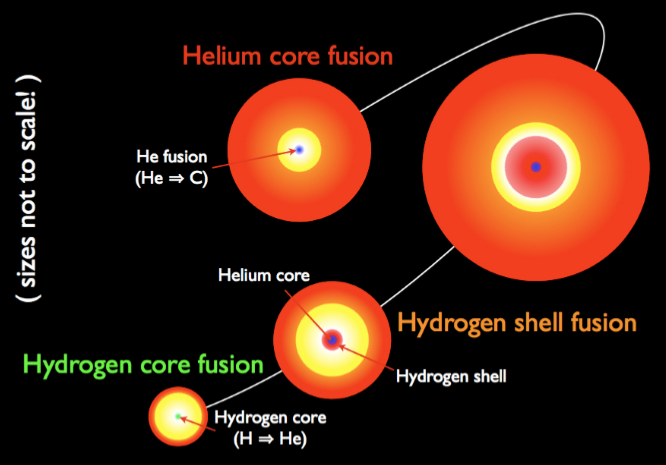
\includegraphics[width=0.7\linewidth]{3}}
	\caption{Изображение ранних этапов эволюции звезд. Звезда начинается со слияния	водорода с гелием. Когда водород в активной зоне истощен, ядро сжимается, что повышает температуру и запускает водородное слияние (!!!fusion) в оболочке вокруг гелиевого ядра. Это расширяет атмосферу звезды и превращает ее в		красного гиганта. После сжигания водородного топлива ядро снова сжимается под 	действием силы тяжести, которая увеличивает температуру до той отметки, при которой синтез начинался. Рисунок из $https://www.nasa.gov/mission\_pages/$}
	\label{ris:3}
\end{figure}

Главное препятствие объединения гелия и водорода в тяжелые элементы - это сильное Кулоновское отталкивание между нуклидами, которые все положительно заряжены. Более того, стандартный способ плавления (!!!!fuse может быть синтез) водороде это p-p цепь, включающая слабую реакцию p + p $\rightarrow$ d + e + + $\nu$e, которая имеет чрезвычайно малое сечение (!!!!!cross section) (Rolfs and Rodney, 1988). Поэтому чрезвычайно высокие температуры ($\&$ 10 MK) являются необходимо для сжигания водорода в гелий и гелий в более тяжелые элементы. Такие условия достигаются внутри звезд, где происходит ядерный синтез (например, Бете 1939), высвобождая энергию ядерной связи в виде тепла, удерживающую звезду от разрушения и заставляя ее сиять.
На рис. \ref{ris:3} изображены ранние стадии эволюции звезд. По определению, каждая звезда, по крайней мере, синтезирует водород в гелий внутри ядра, и звезды проводят большую часть своей жизни в этой фаза горения водорода. Как только запас водорода в ядре исчерпан, температура становится недостаточно высокой для сжигания гелия, поэтому ядро сжимается, потому что источник тепла от сжигания водорода уменьшается. Далее (!!!As the core contracts), он нагревается, и температура становится достаточно высокой для горения водорода в оболочке вокруг гелиевого ядра. В этот момент атмосфера звезды быстро расширяется, и звезда входит в фазу красного гиганта. Когда водород в оболочке исчерпан и, если звезда достигла определенных массы ($\&$ 0,5 М, например, Рольфс и Родни, 1988), ядро снова сжимается, то есть увеличивается температура и становится возможен тройной-альфа процесс, который синтезирует (!!!преобразует) три частицы 4He в 12C. Некоторые гелиевые сплавы также могут быть преобразованы с вновь созданным 12C, чтобы создать 16O, и, в принципе, он также может пойти дальше, производя 20Ne, 24Mg, 28Si и т. д., которые называются альфа-элементами, потому что они являются определенным количество альфа-нуклидов, слитых вместе. Однако на практике реакция 16O + 4He $\rightarrow$ 20Ne является медленной, и поэтому сжигание гелия в основном производит 12C и 16O (см. Rolfs and Rodney, 1988; Hansen et al., 2004). Когда гелий истощается, температура ядра снова повышается за счет сжатия. Наибольшая температура, достигаемая в звезде, зависит от ее начальной массы. Если начальная масса выше ~ 8 М, то углерод и кислород могут быть сожжены, в противном случае звезда заканчивает свою жизнь как углерод-кислородный белый карлик (например, Rolfs and Rodney, 1988; Hansen et al., 2004). Если масса звезда представляет собой лишь несколько солнечных масс выше 8 М, она может быть способна сжигать углерод, а затем стать белым карликом кислорода-неонового цвета.
\subsection{Ядерное горение в тяжелых звездах}

\begin{figure}[h]
	\center{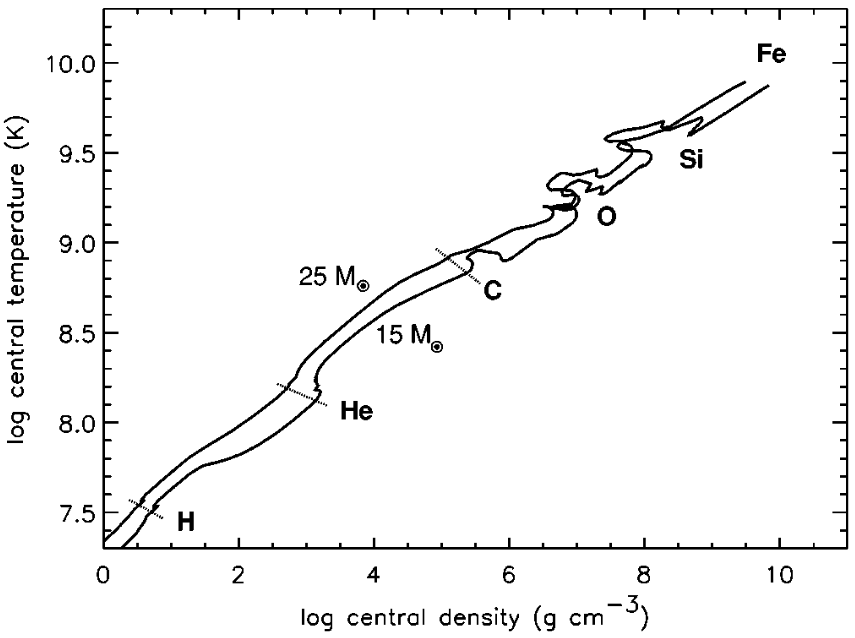
\includegraphics[width=0.7\linewidth]{4}}
	\caption{Центральная плотность и температура 15M, а также 25M звездных моделей. По мере развития звезды центральная плотность и температура возрастают, последовательно воспламеняются водород, гелий, углерод, кислород и сгорает кремний. Рисунок 1 из Woosley et al. (2002) © 2002 Американское физическое общество}
	\label{ris:4}
\end{figure}

Звезды с начальной массой более 8 М проходят через несколько стадий горения. После каждого этапа, ядро сжимается под действием сил тяжести, поскольку ядерное топливо на этой стадии был исчерпано и, следовательно, источник ядерного тепла потерян. Поскольку ядро сжимаются, они нагревается, что позволяет начать следующую стадию горения, если температура будет достаточно высока. Это показано на рис. 1.4 (рис. 1 из Woosley et al., 2002), который показывает центральную плотность и температуру двухзвездной модели и областей, в которых происходят различные стадии горения. В фазе сжигания углерода существуют ряд различных реакции 12C + 12C, но чаще всего наблюдается 20Ne + 4He и 23Na + p. Свободный протон может захватывать другие существующие нуклиды для создания не-альфа-элементов, а также 23Na, являющийся не-альфа-элементом, который могут быть преобразован в другие не-альфа-элементы. Гелий, полученный из сгорания углерода также сжигается как 12C + 4He $\rightarrow$ 16O или 16O + 4He $\rightarrow$ 20Ne. Когда углерод истощается, ядро сжимается до тех пор, пока очень энергичные фотоны (!!!very energetic photons) формирующие хвост Распределения Планка не смогут фото-синтезировать 20Ne, что приводит к образованию свободных альфа-частиц, которые могут захватывать недиссоциированные 20Ne, чтобы сформировать около 24Mg. Реакция с низшим кулоновским барьером теперь 16O + 16O, что в основном приводит к 28Si + 4Не и 31P + p (см. Rolfs and Rodney, 1988). Освобожденные альфа-частицы захватываются на 24Mg и 28Si, чтобы сформировать 28Si и 32S.
В конце сжигания кислорода звездное ядро состоит в основном из 28Si, 32S и небольшого количества других нуклидов. Это является предпосылкой для окончательной фазы горения: сжигание силикона. Перед тем, как температура, требуемая для 28Si + 28Si достигается, кремниевые нуклиды разрушаются фото-диссоциацией, что снова создает источник для свободных альфа-частиц. Эти альфа-частицы захватываются последовательно, начиная с 28Si для создания 32S, 36Ar, 40Ca, 44Ti, 48Cr, 52Fe и 56Ni, что называется альфа процессом или альфа-лестницой, которая встречается на временной шкале (см. Рольфс и Родни, 1988; Hansen et al., 2004). Поскольку температура во время сжигания кремния настолько высока ($\&$ 3,5 ГК), нуклиды, более тяжелые, чем кремний, также могут быть фото-диссоциированными (!!!photodissociated). Результатом являются такие реакции, как 28Si + 4He $\rightarrow$ 32S, которые находятся в равновесии с их обратными реакции. Таким образом, существует группа нуклидов, а именно нуклидов с 28 $<=$ A $<=$ 62, свободные альфа-частицы, нейтроны и протоны, находящихся в равновесии друг с другом. Это состояние называется квазиравновесным (QSE) и отличается от NSE (см. Следующий раздел) тем, что не все нуклиды находятся в равновесии друг с другом. В частности, 12C, 16O, 20Ne, и 24Mg не являются частью группы QSE, описанной выше (например, Bodansky et al.,1968; Woosley et al., 1973).
Однако сжигание кремния могут производить только нуклиды вплоть до атомного массового числа от А = 56, так как энергия связи на нуклон (протоны и нейтроны) достигает максимум при этой массе. Поэтому более тяжелые нуклиды слабее связаны (Rolfs и Rodney, 1988), что означает, что нужно добавить энергию, для обеспечения слияние за пределами A = 56. Другими словами, как только все значимые элементы в ядре массивной звезды сожжены до 56Ni (!!!Ничего не понял), сердцевина звезды будет состоять из ядерной пыли, которая не может гореть, а звезда теряет свой основной источник тепла. Ядро остается поддерживаемым от коллапса давлением вырождения электрона, но как только масса ядра превышает эффективную массу Чандрасекара, происходит коллапс ядра, вызывающий CCSN (например, Woosley et al., 2002). Масса Чандрасекара (~ 1,4 М) является теоретической максимальной масса белого карлика, поддерживаемого только лишь давлением вырождаемости электронов. Однако до того, как железное ядро достигнет массы Чандрасекара, происходит захват электронов нуклидами, которые удаляют электроны и, следовательно, поддерживающее давление, что приводит к коллапсу ядра до того, как оно достигнет массы Чандрасекара. Максимальная масса железного ядра до начала коллапса называется эффективной массой Чандрасекара (например, Woosley et al., 2002). Поскольку звездный синтез по большей части производит альфа-элементы, неудивительно, что мы наблюдаем альфа-элементы, более широко распространенные, чем другие нуклиды ниже пика железа (см. рис. \ref{ris:1}).

\subsection{Пик железа}
Выше температуры (~5GK), реакции слияния уравновешиваются обратной реакцией
фотодиссоциации, что означает, что реакция плавления $N$
нейтронов и $Z$ протонов в нуклиде $(N, Z)$ уравновешивается реакцией расщепления в нуклиде $(N, Z)$ на $N$ свободных нейтронах и $Z$ свободных протонах. Такое состояние называется nuclear statistical equilibrium (NSE). Когда материя находится в состоянии NSE, весь состав, т. е. концентрация каждого вида ядра, полностью определяется температурой, плотности и электронной частью $Y_e = n_p/(n_p + n_n)$, где $n_p$ - общая плотность протонов (свободных или внутри нуклидов), а $n_n$ - аналогичное значение для нейтронов (например, Seitenzahl et al. ., 2009).

Нуклиды, которые более тесно связаны будет более распространены, чем нуклиды, которые менее связаны, так как их нуклиды труднее разбить фотодиссоциацией, и поэтому равновесие оставит такие нуклиды не тронутыми. По этой причине распределение NSE благоприятствует нуклидам в районе A = 56, т.е. пик железа, поскольку они являются наиболее тесно связанными нуклидами. Это справедливо только в том случае, если $Y_e$ близко к 0,46, что представляет собой долю электронов 56 $F_e$, а также только в том случае, если температура не слишком велика (с учетом плотности), поскольку в противном случае NSE будет способствовать свободным нейтронам и протонам (например, Seitenzahl et al., 2009).

Такие условия достигаются в сверхновой типа $Ia$, где белый карлик, состоящий в основном из углерода и кислорода, подвергается термоядерному взрыву. Последующее нагревание заставляет материю перейти в состояние NSE, которое порождает пики железа нуклидов, которые будут сохраняться после того, как материал снова остынет

\begin{figure}[h]
	\center{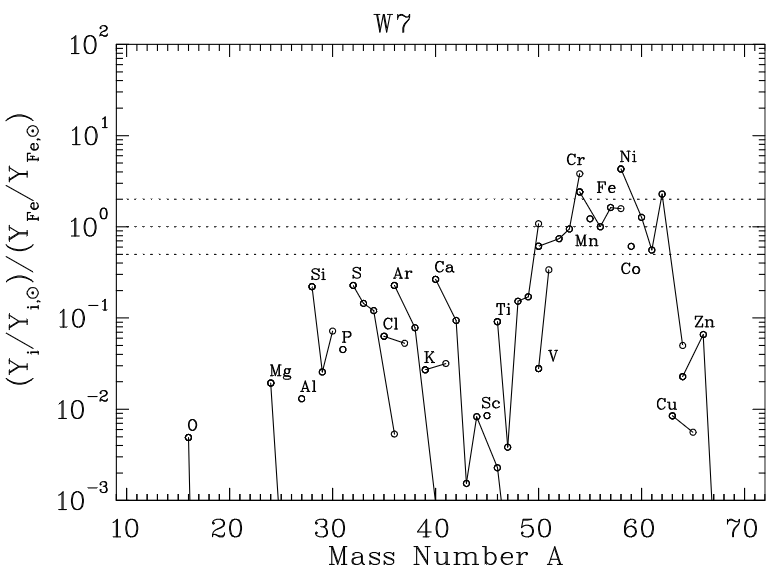
\includegraphics[width=0.7\linewidth]{5}}
	\caption{Конечные показатели концентрации в модели сверхновой типа $Ia$. В основном наблюдаются элементы железного пика, а также некоторые тяжелые альфа-элементы (кремний, сера, аргон, кальций и титан)}
\end{figure}

Рисунок \ref{ris:5} (рис. 12 из Iwamoto et al., 1999) показывает конечную концентрацию из модели сверхновой звезды типа $Ia$. Тип $Ia$ сверхновых вносит значительный вклад в формирование пика железа вместе с горением кремния вр время CCSNe и медленного захвата электронов (см. следующую главу) в тяжелых звездах (см. Timmes et al., 1996; Woosley et al., 2002)


\newpage 
!!!Возможно что то пропущено, проверь
\newpage
\subsection{Нуклеосинтез за пиком железа}
Поскольку процесс слияния становится эндотермическим для A $\ge$ 56, а кулоновский барьер становится
непреодолимо большим, требуется другой процесс для создания элементов за пределами железного пика. Этот процесс представляет собой захват нейтронов, который остается экзотермическим до тех пор, пока энергия связи нейтронов Qn остается большой для ядер, богатых нейтронами. В некоторой точке, $Q_n$ настолько мала (~ 1 МэВ), что показатель фоторасщепления (фотонный выброс нейтрона из ядра) так же велик, как и показатель захвата нейтронов, и поэтому нет оставшихся нейтронов, связанными с ядром. Момент, в который это происходит называется нейтронной капельной линией (!!! neutron drip line) и, как правило, составляет 10-20 нейтронов, превышающих наиболее богатый нейтронами стабильный изотоп (например, Rolfs and Rodney, 1988). Точное положение нейтронной капельной линии зависит от температуры и плотности нейтронов. Очевидно, что Кулоновский барьер  для захвата нейтронов отсутствует, поскольку нейтроны имеют нейтральный заряд.
Как только ядро захватывает нейтрон, оно может оставаться стабильным, и в этом случае оно может захватить другой нейтрон, но в большинстве случаев новый нуклид будет неустойчивым к $\beta$-распаду.

Важным отличием является то, что временная шкала $\tau\beta$ для $\beta$-распада короче или длиннее чем временная шкала $\tau_n$ для захвата нейтронов. Если $\tau_\beta << \tau_n$, то каждый неустойчивое ядро, созданное захватом нейтронов, распадется до стабильного ядра, прежде чем у него появится шанс захвата другого нейтрона. Следовательно, процесс захвата нейтронов медленный по сравнению с $\beta$-распадом, и поэтому это называется процессом захвата медленных нейтронов или s-процессом (!!!туту что то не то). S-процесс никогда не дестабилизирует более одного ядра и, следовательно, протекает вдоль области устойчивости (область на карте нуклидов, где ядра стабильны, обозначена квадратами на рис. 1.6). Если, с другой стороны, $\tau_\beta \gg \tau_n$, то есть время для множественных захватов нейтронов до первого $\beta$-распада. Это называется процессом захвата быстрых нейтронов или r-процессом (то же самое), поскольку захват нейтронов происходит быстро. В этом случае нуклеосинтез протекает вдоль нейтронной капельной линии, но он вынужден дождаться $\beta$-распада в этой точке (например, Rolfs and Rodney, 1988)

\begin{figure}[h]
	\center{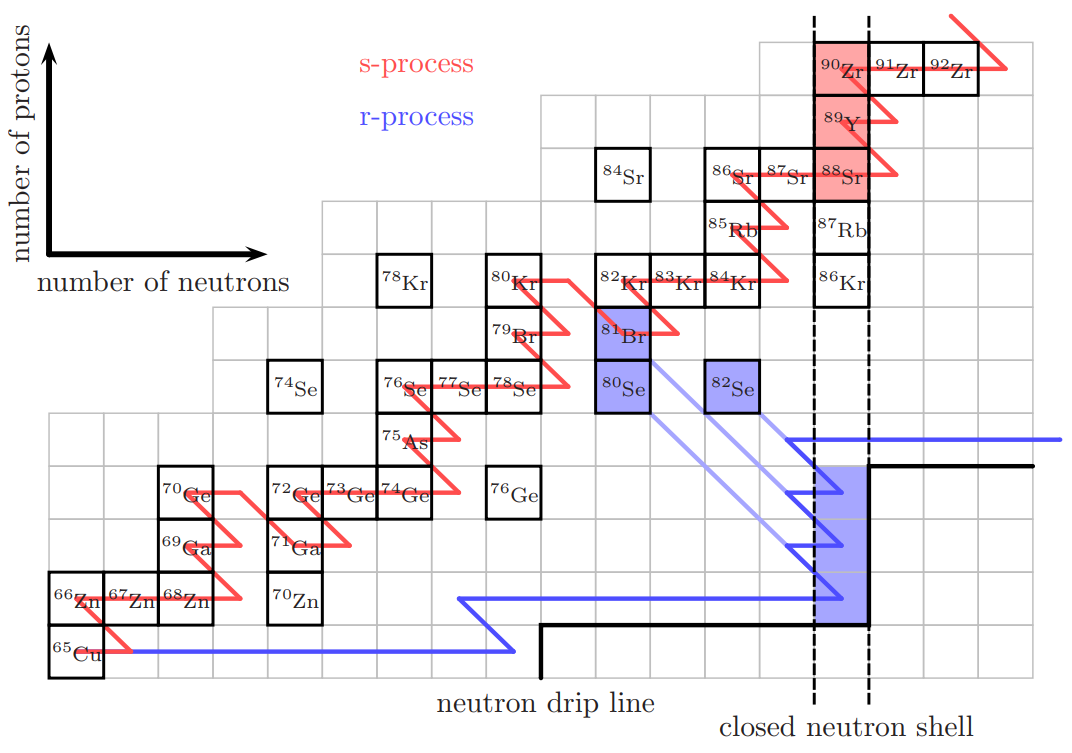
\includegraphics[width=0.7\linewidth]{6}}
	\caption{Схематическое представление s- и r-процесса на участке диаграммы нуклидов. S-процесс (красный) проходит вдоль долины устойчивости и r-процесс (синий) вдоль линии капельного потока нейтронов. На закрытой нейтронной оболочке N = 50 сечение захвата нейтронов падает на несколько порядков, что приводит к накоплению материала, который производит двух-пиковые характеристики, показанные на рисунке 1.1}
	\label{ris:6}
\end{figure}

На рис. \ref{ris:6} схематично показаны пути s- и r-процессов на участке диаграммы нуклидов.Если ядро имеет определенной количество нейтронов, называемое магическим числом, то нейтроны могут быть расположены в замкнутой оболочке, которая энергетически очень благоприятна и резко уменьшает сечение захвата нейтронов (Rolfs and Rodney, 1988). Это показано на рисунке 1.6 при N = 50. Когда r-процесс достигает замкнутой нейтронной оболочки, ему приходится ждать, пока произойдет несколько $\beta$-распадов могут протекать мимо закрытой нейтронной оболочки. Поэтому материал будет накапливаться там, где нейтронная капельная линия пересекает замкнутую нейтронную оболочку, обозначенную квадратами на рис. \ref{ris:6}. Поскольку эти нуклиды все нестабильны, они в конечном итоге распадаются до состояния устойчивости когда все свободные нейтроны будут захвачены, а избыток материала, который был получен на закрытой нейтронной оболочке, приведет к пику обилия в массе, где нуклиды имеют меньше нейтронов, чем магическое число (потому что некоторые нейтроны распались на протоны). Аналогичным образом, когда s-процесс пересекается с закрытой нейтронной оболочкой, также будет избыток материала но не потому, что s-процесс должен ждать дополнительных $\beta$-распадов (напомним, что $\beta$-распады всегда происходят намного быстрее, чем захват нейтронов s-процесса). Материя накапливается на закрытой нейтронной оболочке, поскольку сечение захвата нейтронов на один-два порядка меньше, чем для соседних нуклидов (Рольфс и Родни, 1988). Таким образом, s-процесс будет порождать пики обилия в тех массах, где число нейтронов - это в точности магическое число, которое является большей массой, чем пики, образуемые r-процессом. Наиболее важные магические числа это N = 50; 82; 126, которые приводят к пикам распространенности при приблизительно A = 80; 130; 194 для r-процесс и около A = 88; 138; 208 для s-процесса. Рисунок 1.7 (Рисунок 1 от Arnould et al., 2007) показывает вклад s- и r-процессов в солнечных концентрациях. Пики с разными значениями массы также хорошо видны (особенно второй и третий), как показано на рисунке 1.1. Когда мы исследуем r-процесс, мы всегда сравниваем предполагаемое обилие с образцом солнечного r-процесса, показанном на рисунке 1.7. Оказывается, что пример обилия r-процесса является универсальным и имеет то же относительное обилие, что и в Солнце, наблюдаемое в гало звезд с недостатком металла (!!!Ужас просто) (например, Sneden et al., 2008; Roederer et al., 2010). Обилия R-Process'а из пяти таких звезд показаны на рис. 1.8, см. Рисунок 8 от Sneden et al. (2009). Звезды с ореолам, бедными металлами, сформировались на ранней стадии жизни нашей галактики, и поэтому мы ожидаем, что они не будут значительно обогащены тяжелыми элементов, созданных s-процессом, поскольку у него не было достаточного времени для образования этих звезд (см. также раздел 1.5). Поэтому любая реалистическая модель нуклеосинтеза r-процесса должна воспроизводить обилия солнечного r-процесса показанного на рисунке 1.7.

\begin{figure}[h]
	\center{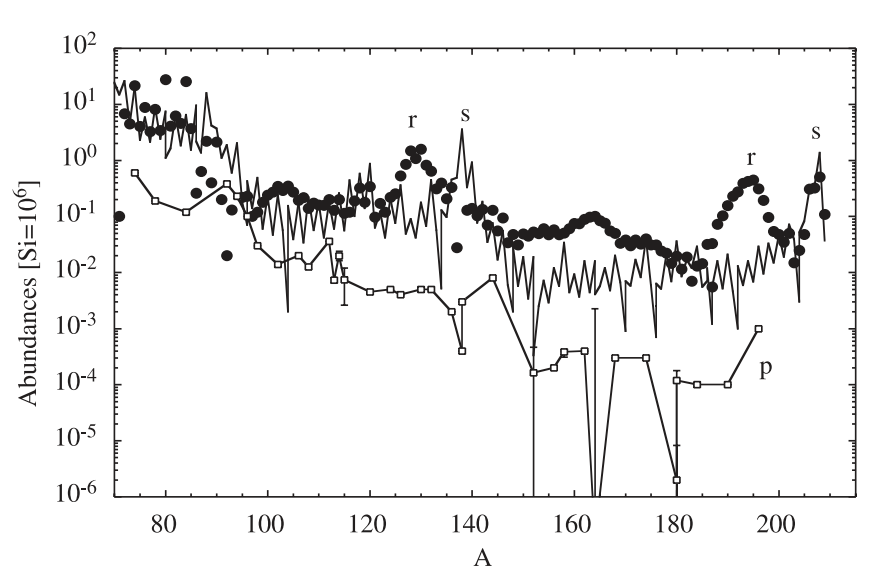
\includegraphics[width=0.7\linewidth]{7}}
	\caption{Вклад s-процесса (сплошная линия), r-процесс (точки) и p-process (квадраты) в изобилиях Солнца. Заметим, что r-процесс создает пики при несколько меньших массах, чем s-процесс. Рисунок 1 от Arnould et al. (2007)}\label{ris:7}
\end{figure}

\begin{figure}[h]
	\center{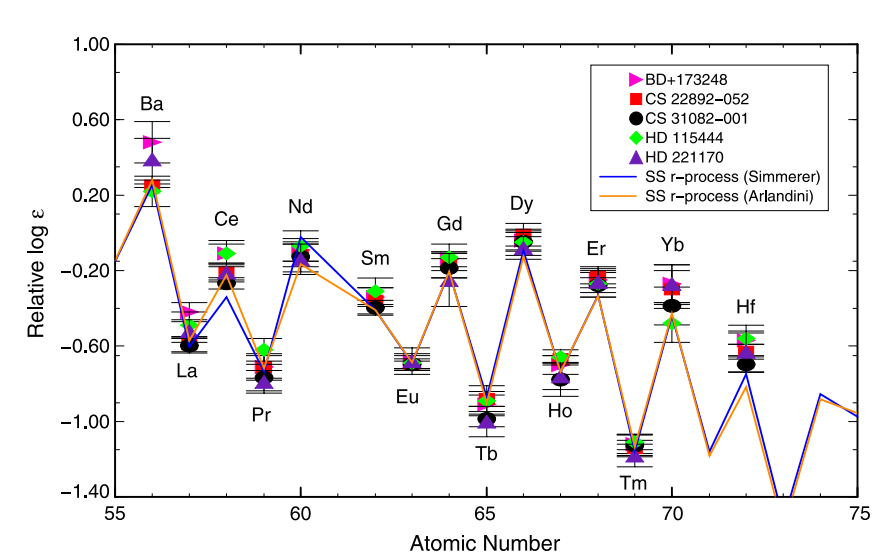
\includegraphics[width=0.7\linewidth]{8}}
	\caption{Наблюдаемые обилие некоторых тяжелых элементов в пяти металлически-бедных ореолах
		звезд. Обилие нормируется в европиуме. Все звезды имеют практически одинаковые относительные количества, и эта картина также согласуется с тем, что наблюдается в		солнечной системе (линии). Ожидается, что эти звезды не будут обогащены s-процессом нуклеосинтеза, потому что они образовались вскоре после образования галактики. Следовательно, это вывод показывает, что r-процесс создает универсальную картину обилия. Рисунок	8 от Sneden et al. (2009)}
	\label{ris:8}
\end{figure}

На рис. 1.7 также показан вклад p-процесса в изобилиях Солнца, который на несколько порядков меньше вкладов s- и r-процессов. P-процесс производит нуклиды на богатой протонами стороне области стабильности (например, 74Se, 78Kr и 84Sr на рис. 1.6). P-процесс - это активная область исследований, которая еще не совсем понятна. Это может быть возможно в массивных звездах в их пред-сверхновой фазе и всех типах сверхновых. См. Arnould and Goriely (2003) для современного и всестороннего обзора.

Наконец, некоторые авторы также рассматривают процесс промежуточного захвата нейтронов, называемый
i-процесс, между медленным и быстрым процессами. I-процесс протекает на богатой нейтронами стороне, и дестабилизирует до пяти нуклидов (например, Cowan и Розе, 1977; Bertolli et al., 2013). S-процесс и/или i-процесс происходят внутри звезды с низкой массой асимптотической гигантской ветви (AGB) (1: 5? M? M? 3), а также более массивных звездах, которые, как правило, имеют сильные звездные ветра, которые выделяют некоторые из вновь созданных тяжелых элементов в межзвездную среду (например, Peters, 1968; Couch et al., 1974; Käppeler et al., 1994; Woosley et al., 2002; Straniero et al., 2006; Гервиг et al., 2011). Реакции 13C + 4He! 16O + n и 22Ne + 4He! 25Mg + n приводят к появлению свободных нейтронов. Астрофизические условия (!!!site) r-процесса остаются открытыми вопросами и являются предметом следующего раздела.

\subsection{Возможные места r-процесса}

Для r-процесса требуется очень богатая нейтронами среда. Было предложено множество мест, в которых могут быть достигнуты правильные условия для r-процесса. К ним относятся ударные или струйные выбросы в сверхновых, богатых нейтронами, неоднородные космологии Большого Взрыва, выбросы от коалесценции и приливного разрушения бинарных нейтронных звезд, выбросы (!!!nova outburst), взрывчатого гелия или сжигание углерода, вспышки гелиевых ядер в звездах с низкой массой, или аккреционные диски нейтронной звезды (см. Mathews and Cowan, 1990, и ссылки в нем). Основываясь на наблюдениях европия в звездах с небольшим содержанием металла и галактических моделях химической эволюции , Мэтьюз и Коуэн (1990) пришли к выводу, что CCSN были наиболее вероятным местом протекания r-процесса. Недавние исследования показывают, что CCSN и слияние нейтронных звезд являются единственными жизнеспособными кандидатами на сайт r-процесса (например, Thielemann et al., 2011).

\subsection{Коллапс ядра сверхновых}

После коллапса железного ядра массивной звезды образуется прото-нейтронная звезда (PNS). Эта PNS делептонизирует, чтобы в конечном итоге сформировать нейтронную звезду. Этот процесс испускает порядка $10^{53}$ эрг
энергии связи в виде нейтрино. Это большое облучение нейтрино приводит к горячему ветру с поверхности ПНС, называемому ветром, управляемым нейтрино (!!!neutrino-driven wind) (например, Цянь и Вусли, 1996). Ранние симуляции и модели этого ветра показывали, что в некоторых случаях они могут иметь хорошие условия для r-процесса (например, Woosley et al., 1994; Wanajo, 2006).

\begin{figure}[h]
	\center{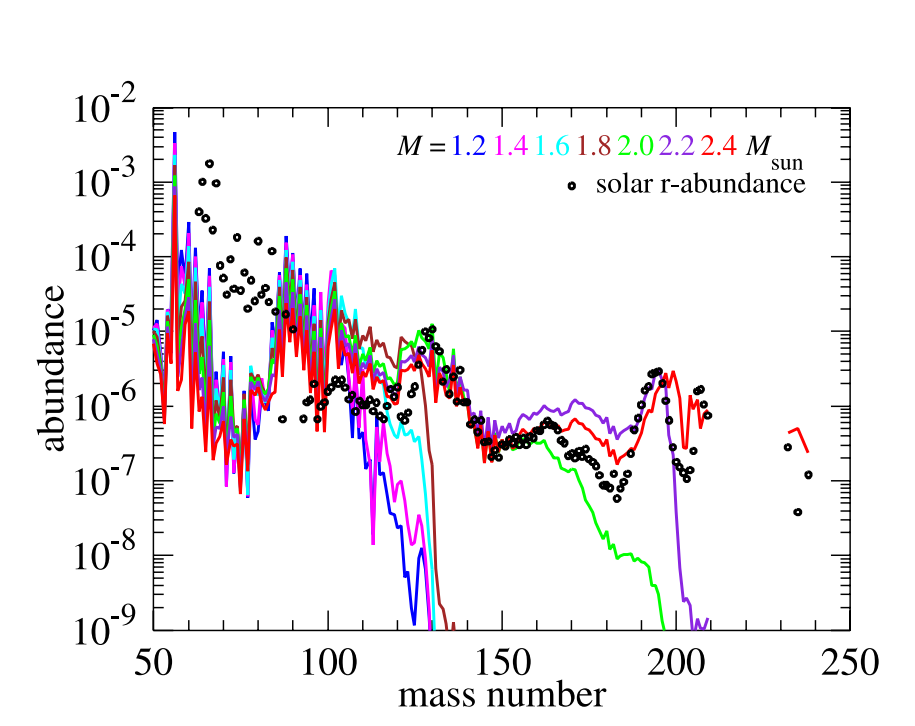
\includegraphics[width=0.7\linewidth]{9}}
	\caption{Конечные посчитаные распространенности нуклеосинтеза r-процесса в ветер с нейтрино от PNS во время CCSN. Показаны обилия как функция от массы PNS. Чтобы получить полный r-процесс до третьего пика (A? 195), требуется M  2 M, что нереально на основе наблюдаемого распределения массы нейтронных звезд. Однако для меньших масс PNS r-процесс устойчиво синтезирует элементы до A? 130.}
	\label{ris:9}
\end{figure} 

Однако последние исследования нуклеосинтеза r-процесса в ветрах с участием нейтрино показали, что маловероятно, что r-процесс полностью (получение нуклидов до третьего пика, см. Рис. 1.1) протекает в этих условиях, поскольку ветер похоже, недостаточно богат нейтронами. Получается, что только слабая версия r-процесса (получение тяжелых элементов до A? 130) может происходить в ветре с нейтрино от CCSNe (например, Qian and Woosley, 1996; Thompson et al., 2001; Fischer et al., 2010; Roberts et al., 2010; Martínez-Pinedo и др., 2012; Wanajo, 2013). Рисунок 1.9 (рис. 8 из Wanajo, 2013) показывает расчет r-процесса нуклеосинтез в ветре с участием нейтрино от CCSN.

Однако существует еще один процесс, так называемый «$\nu р$-процесс», который может создавать нуклиды до $А~110$ в насыщенном протоннами ветре с участием нейтрино. В горячем, богатом протонами ветре, захват протонов создает богатые протоном ядра, но прекращается при 64Ge, который имеет долгий $\beta$ - период полураспада (? 64 с) по сравнению с расширенной временной шкалой (? 10 с) и малого сечение захвата протоннов. $\nu p$-процесс может пройти через этот 64Ge барьер путем преобразования свободного протона в нейтрон посредством электронного антинейтринного захвата. Реакция 64Ge + n! 64Ga + p намного быстрее, чем захват протонов на 64Ge и позволяет нуклеосинтезу протекает через A = 64 с последующими захватами протонов (например, Fröhlich et al., 2006; Pruet et al., 2006; Wanajo и др., 2011; Arcones et al., 2012).

\begin{figure}[h]
	\center{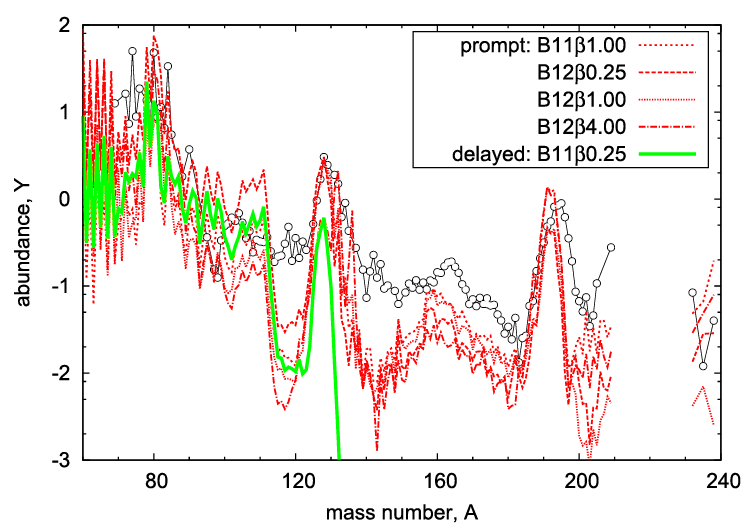
\includegraphics[width=0.7\linewidth]{10}}
	\caption{r-Процесс нуклеосинтеза приводит к особому типу CCSN, управляемому магнитосопротивлением (!!!magnetorotationally). Этот тип сверхновой может производить полный r-процесс до третьего пика, но из-за большого магнитного поля и степени вращения, которые требуются,  можно сказать, что это будет очень редкий (.0: 1$\%$) класс CCSN.}
	\label{ris:10}
\end{figure}

Наконец, определенный редкий тип CCSNe может иметь возможность обеспечивать полный r-процесс. Если звезда-предшественник имеет сильное магнитное поле, и ее ядро вращается быстро, тогда взрыв сверхновой может приводиться в действие магнитороциональными (!!!magnetorotational) процессами (возможно магнитореформационная неустойчивость), которые могли создать биполярную струю (см., Уилер et al., 2000; Akiyama et al., 2003; Burrows et al., 2007; Mösta et al., 2014, 2015). Возможно, что в этой струе имеет место r-процесс нуклеосинтеза (например, Winteler et al., 2012; Nishimura et al., 2015), который создает все тяжелые элементы до третьего пика. На рис. 1.10 показан расчет нуклеосинтеза r-процесса в таких магнитно-зависимый(!!!magnetorotational) CCSN от Nishimura et al. (2015, их рисунок 13). Однако, из-за огромного магнитного поля и быстрого вращения, требуемого в этом типе суперновых, ожидается, что только малая доля (0,1: 1) из всех CCSNe приводит к созданию магниторотационной сверхновой (Nishimura et al., 2015).

\begin{figure}[h]
	\center{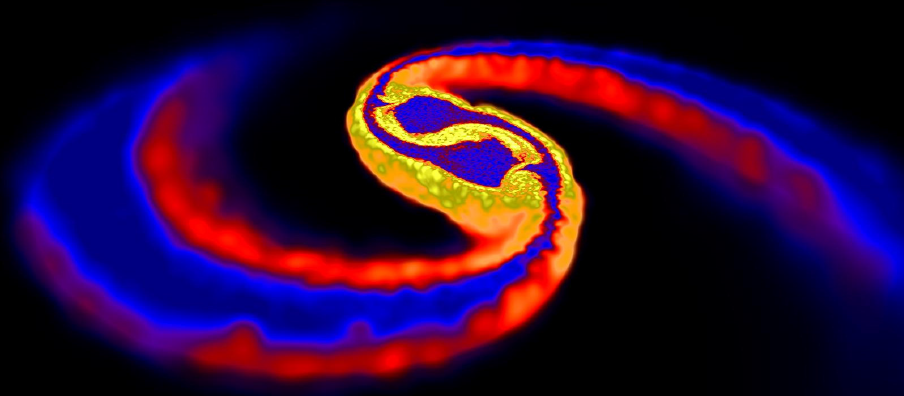
\includegraphics[width=0.7\linewidth]{11}}
	\caption{Плотностный рендеринг моделирования слияния двойных нейтронных звезд. Темные центральные капли - это две нейтронные звезды перед слиянием. Динамические выбросы богатого нейтронами вещества в виде двух приливных хвостов отчетливо видны. Этот материал является несвязанным, а также в нем происходит r-process}
	\label{ris:11}
\end{figure}

Поскольку обычный CCSN, скорее всего, не может произвести полный r-процесс, остается только слияние нейтронных звезд как единственное жизнеспособное место для нуклеосинтеза r-процесса. Мы знаем, что в нашей галактике существуют бинарные системы нейтронных звезд, и, что их орбита сокращается из-за излучения гравитационной волны (например, Hulse и Taylor, 1975; Lattimer и Prakash, 2005), что приведет в результате к объединению двух нейтронных звезд (например, Price и Rosswog, 2006). Множество групп провели гидродинамическое моделирование слияния двух нейтронных звезд или слияние нейтронной звезды и черной дыры. Такие слияния могут выбрасывать богатый нейтронами материал через различные процессы. Существует два типа динамических выбросов, которые запускаются незадолго до или во время слияния. Поскольку две нейтронные звезды приближаются друг к другу или одна нейтронная звезда приближается к своей черной дыре, нейтроная звезда(ы) получает ... (приливной) tidally деформируется и разрушается, что создает поток материи нейтронной звезды, выброшенный в космос и несвязанный с системой (см., Price и Rosswog, 2006; Foucart et al., 2014; Sekiguchi et al., 2015; Kyutoku et al., 2015; Radice et al., 2016). Этот тип выброса относится к приливным хвостам. Пример показан на рисунке 1.11. Второй тип динамических выбросов - сжатие материи при столкновении между двумя нейтронными звездами. Этот тип динамических выбросов происходят только при слияниях нейтронная звезда - нейтронная звезда (NSNS) (например, Bauswein et al., 2013; Hotokezaka и др., 2013b). Масса динамического выброса находится от 10-4 до нескольких 10-2 массы Солнца и распределение электронной доли колеблется от $Y_e ~$ 0.05-0.45 в случае бинарных нейтронных звезд. Черные дыры-нейтронные звезды могут выбросить порядка $~$0.1 М, но только если черная дыра имеет такую ??же массу, как нейтроная звезда и имеет довольно высокий уровень вращения. Иначе, как правило, нет выброса вообще, потому что нейтронная звезда разрушается внутри горизонта событий черной дыры. Доля электронного выброса от слияния BHNS обычно ниже 0,2 (Foucart et al., 2014). Я обсуждаю нуклеосинтез r-процесса в динамических выбросах BHNS слияние подробнее в главе IV.

\begin{figure}[h]
	\center{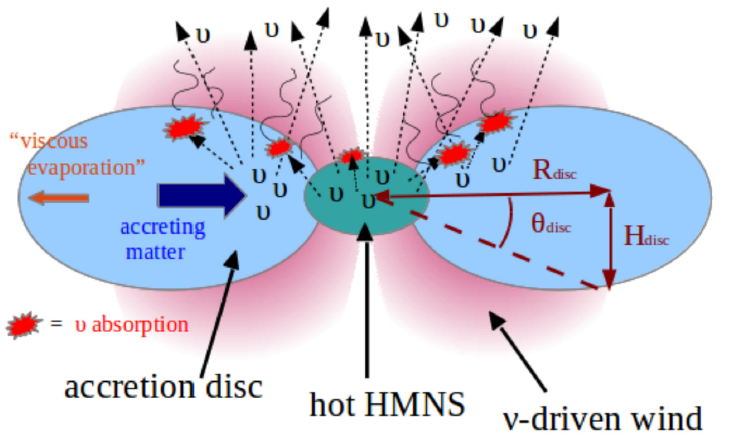
\includegraphics[width=0.7\linewidth]{12}}
	\caption{Изображение аккреционного диска вокруг HMNS и возникающий в результате нейтринный вет}
	\label{ris:12}
\end{figure}

Слияние нейтронных звезд может привести к дополнительным оттокам после слияния. В большинстве случаев вокруг центрального компактного объекта, который является либо черной дырой, либо горячей гипермассивной нейтронной звездой (HMNS) образуется аккреционный диск или тор. Время жизни HMNS до того, как оно схлопнется до черной дыры, колеблется от нескольких миллисекунд до более 30 мс (см., Sekiguchi et al., 2011; Hotokezaka et al., 2013a). Если есть HMNS, она будет излучать нейтрино. Горячий аккреционный диск также охлаждается через излучение нейтрино. Это может привести к ветру с нейтрино с поверхности диска, см. Рис. 1.12 (рис. 1 из Perego et al., 2014). Отток с диска также может быть вызван вязким нагревом и альфа-рекомбинацией на диске. Поскольку этот отток происходит в более поздние времена, облучение нейтрино имеет достаточно времени для значительного повышения электронной доли в оттоке, так что большинство симуляций обнаруживают Ye? 0: 2 ?? 0:45 с несколькими? 10??3M выбрасываемыми в эти оттоки диска (например, Surman et al., 2008; Wanajo and Janka, 2012; Fernandez and Metzger, 2013; Perego et al., 2014; Just et al., 2015; Foucart et al., 2015 ). r-Процесс нуклеосинтеза в оттоке диска после слияния NSNS является предметом главы V.

Поскольку выбросы от слияния нейтронной звезды настолько богаты нейтронами,  r-процесс может легко создать все элементы до A? 250, что выходит за пределы третьего пика. По факту, во время r-процесса нуклеосинтеза образуются еще более тяжелые нуклиды (A> 300) однако эти нуклиды нестабильны для деления (как спонтанные, так и нейтронно-индуцированные). Их продукты деления быстро захватывают больше нейтронов, растут до A> 300, а затем делятся сами собой. Этот так называемый цикл деления продолжается до тех пор, пока нейтроны не будут исчерпаны. Замечательный результат заключается в том, что окончательная картина обилие r-процесса очень устойчив к вариациям в дтелизации свойств выброса. Если цикл деления начался, то конечная численность не будет зависеть от точного числа циклов (см., Korobkin et al., 2012; Bauswein et al., 2013; Mendoza-Temis et al., 2015). Рисунок 1.13 (рис. 4 от Korobkin et al., 2012) показывает результат r-процесса нуклеосинтеза в различных слияниях NSNS и BHNS. Все сценарии слияния производят по существу идентичные конечные распространенности, демонстрируя тем самым устойчивость r-процесса в слияниях нейтронных звезд.

\subsection{Химическая эволюция галактики}

Несколько групп показали устойчивость нуклеосинтеза r-процесса в слияниях нейтронной звезды, которые очень хорошо отражают закономерности обилия, соответствующие наблюдаемой картине солнечного r-процесса (например, Freiburghaus et al., 1999; Goriely et al., 2011; Wanajo et al. , 2014; Goriely et al., 2015; Just et al., 2015; Radice et al., 2016). Но еще есть некоторые проблемы, которые необходимо решить до того, как слияние нейтронных звезд может быть принято в качестве основного места r-процесса (например, Qian, 2000; Argast et al., 2004; Matteucci et al., 2014). Эти проблемы связаны с наблюдениями материалов r-процесса у очень бедных металлом звезд, которые были сформированы на раннем этапе жизни галактики, и наблюдением небольшого разброса в обилиях r-процесса в галактике.

Предполагается, что галактика образуется из первозданного газа, содержащего только водород и гелий. Когда звезды формируются, эволюционируют и умирают при взрывах сверхновых, межзвездный газ обогащается более тяжелыми элементами, в частности железом. Из этого обогащенного газа образуются новые звезды, которые начинаются с некоторых тяжелых элементов (тяжелее гелия).


\subsection{!!!Вышел из введения во вторую главу (Self-heating evolution)}
\subsection{Эволюция само-нагрева}
В предыдущем разделе мы продемонстрировали, как SkyNet получает ядерные обилия во времени, если и температура, и плотность заданы как функции времени. В большинстве случаев используется история плотности $\rho(t)$ (например, когда используется SkyNet для пост-процесса нуклеосинтеза для слежения за частицами из гидро-симуляции), но температура не обязательно известна как функция времени. И даже если у нас есть информация о изменении температуру, она, скорее всего, не включала бы нагревание (!!!) из-за ядерных реакций, которые развивается SkyNet. Но основываясь на описание кинетической теории уравнений реакционной сети (!!!the kinetic theory description of the reaction network equation) в разделе 2.2.1, а также обсуждение подробного баланса в разделе 2.2.3, становится ясно, что реакционная сеть и термодинамическое состояние жидкости тесно связано и требует последовательной обработки. Следовательно, мы хотим, чтобы температура развивалась в сети под влиянием ядерных реакций, которые выделяют ядерную энергию связи в виде тепла. Это известно как эволюции само-нагревающейся сети (например, Freiburghaus et al., 1999). Нам все еще требуется определить плотность как функцию времени.
Исходя из первого закона термодинамики,
$$
dU = \sigma Q - \sigma W = \sigma Q - P dV
$$
де $dU$ - бесконечно малое изменение внутренней энергии, $\sigma Q$ - бесконечно малая теплота, добавленная в систему из окружающей среды, а $\sigma W$ - бесконечно малая механическая работа, выполняемая системой. Если система расширяется или сжимается, проделанная работа имеет вид $\sigma W = PdV$, где P - давление, dV - бесконечно малое изменение объема. Мы используем энтропию S, объем V и композицию ${N_k}$ как независимые термодинамические переменные. Заметим, что индекс k пробегает все частиц в системе, а не только нуклиды. Полный дифференциал внутренней энергии таким образом:
$$(2.42)$$
где T - температура, $\mu k$ - химический потенциал частицы k. Приравнивание
Уравнение (2.41) и уравнение (2.42) дают
$$2.43$$
Если мы разделим уравнение выше на NB, общее количество барионов и заменим бесконечно малые изменения на разницу величин от одного временного шага к следующему (т. Е.
$\Delta X = X(t + ?t) - X(t)$, находим
$$2.44$$
так как $Y_k = N_k / N_B$ (уравнение 2.13). Заметим, что сумма над k включает в себя все частицы,
следовательно, и электроны, которые могут быть созданы или разрушены при слабых ядерных реакциях.
$\Delta q$ - изменение теплоты на барион от внешних источников тепла. Пусть $2.45$ будет  внешнюю скорость нагрева (на барион), тогда
$$(2.45)$$.
где $...$ - скорость нагрева / охлаждения нейтрино системы в окружающей среде по уравнению (2.194). Поскольку мы не включаем нейтрино во внутреннее состояние система, нейтринное нагревание / охлаждение следует рассматривать как внешний источник тепла. И поскольку мы определяем $...$ как нагрев / охлаждение окружающей среды, он имеет знак минус в уравнении (2.44). Объединение уравнения (2.44) с уравнением (2.45) и решая его для ?s, получаем
$$2.46$$
где мы использовали уравнение (2.128) и переключились на индекс i, который проходит только по нуклидам. Поэтому мы явно включаем вклад электронов $Z_i$, которые взаимодействуют с нуклидом i. Чтобы сделать остальные массовые члены в сумме, близкой к единице, определим массовый избыток $M_i$ как
$$2.47$$
где $A_i$ - число нейтронов и протонов видов i, а $m_u$ - атомная массовая единица, определенная таким образом, что избыток массы $^{12} С$ равен 0 (т. е. $mu = m_{^{12}C} / 12$). Поскольку $Y_i = N_i / N_B$ (с $N_i$, являющимся частицами вида $[i]$, см. Уравнение 2.13), мы получаем
$$2.48$$
потому что частицы вида $[i]$ состоят из $A_i$ нейтронов и протонов, следовательно, $A_i$-барионов. таким образом мы имеем $...$ для всех времен t, что является еще одним способом сказать, что общее барионное число $N_B$ сохраняется. Используя это, мы находим
$$2.49$$
Исходя из вышеизложенного и тото факта, что $n_i=Y_i n_B$, мы можем записать уравнение (2.46) как
$$2.50$$
Обратите внимание, что внешний нагрев учитывается с помощью метода Эйлера первого порядка. Мы планируем улучшить это в будущем, когда мы реализуем более высокий порядок интеграции для самой сети. С учетом вышеизложенного SkyNet может обновлять энтропии после каждого временного шага, а затем получить новую температуру в конце каждого временного шага от EOS. Поэтому нам нужно знать только начальную энтропию (или температура, из которой определяется энтропия). Это немного меняет эволюцию (Уравнение 2.37), так как теперь мы должны использовать энтропию в начале временного шага для оценки температуры в конце временного шага. То есть, мы
решаем
$$(2.51)$$
где $T*$ получено из EOS как
$$(2.52)$$
Уравнение (2.51) решается методом NR, как описано в предыдущем разделе. Заметим, что $\Delta t$ фиксируется в течении итераций NR, что означает температура и плотность также фиксированы. После того, как итерации NR сошлись, мы нашли новые количества $Y_i(t + \Delta t)$, а затем мы можем вычислить $\Delta s$ согласно уравнению (2.50) и обновить энтропию как
$$(2.53)$$
Следовательно, мы имеем гибридную неявную / явную схему, в которой обилия развиваются неявно, но энтропия развивается явно. Можно было бы также эволюционировать энтропию неявно вместе с обилиями, которые потребует вычисления $...$ и $...$ и добавив эти термины к якобиану. Мы можем расширить SkyNet в будущем для поддержки полностью неявной схемы, но пока что мы достигли хорошего результаты с гибридным подходом.
Энергия, выделяемая в ядерной энергии связи из-за ядерных реакций,
$$(2.54)$$
где мы использовали Уравнение (2.49) и $\Delta Y_i / \Delta t$ - приближение для $...$ за шаг. Обратите внимание, что знак минус исходит из того, что избыток массы преобразуется в энергию, поэтому скорость нагрева является положительной, если есть чистое (!!!net) сокращение в избыток массы. Некоторые авторы (например, Hix and Thielemann, 1999) рассматривают $...$ как внешний источник тепла. Это необходимо, если EOS не зависит от всей композиции но только от A и Z, например, средние массы и зарядовые числа. Для сравнения ядерное нагревания в SkyNet с другими программами, SkyNet вычисляет и записывает полную скорость нагрева $...$, независимо от того, включено ли самонагревание. $Utot$ вычисляется как
$$(2.55)$$
Обратите внимание, что вышеприведенное имеет единицы erg $s^{-1}$ $baryon^{-1}$, чтобы преобразовать его в более частое используемых единиц erg s-1 g-1, мы просто умножаем $...$ на константу Авогадро ($N_A$).
В настоящее время SkyNet записывает общую скорость нагрева, показанную выше. В действительности эта скорость нагрева состоит из нескольких компонентов, термализованных в материале в различными способами (например, Barnes et al., 2016). Например, испускаемые электроны и позитронов, а также кинетическая энергия осколков деления, термализованная с очень высокой эффективность, тогда как лишь небольшая часть энергии, высвобождаемой как нейтрино, может термализовать. В будущей версии SkyNet мы планируем записать различное показатели нагревания так что термализация может быть учтена в кило-нова свете расчете кривых, напрмер.

\subsection{2.3.3 Критерий сходимости и временной шаг}
\begin{figure}[h]
	\center{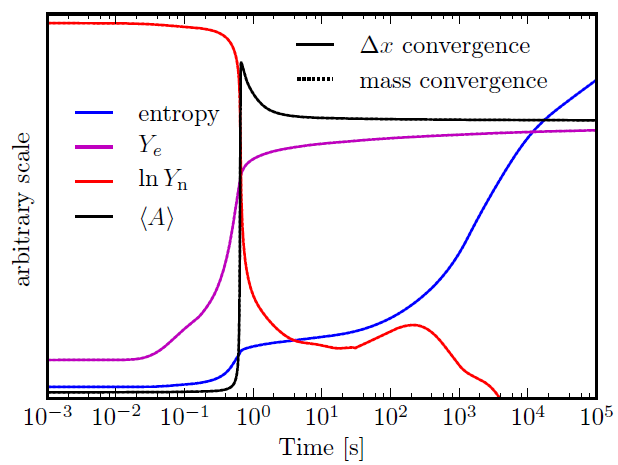
\includegraphics[width=0.7\linewidth]{21}}
	\caption{Сравнение двух критериев сходимости. Сплошные линии показывают энтропии, электронные доли $Y_e$, логарифм численности нейтронов $Y_n$ и среднее массовое число <A> как функции времени с использованием критерия сходимости $\Delta x$ (Уравнение 2.56) с $"tol;? X = 10??6$. Пунктирные линии, построенные сверху сплошных линий, являются соответствующими величинами с использованием критерия сходимости сохранения массы (уравнение 2.57) с $...$. Для всех величин две линии находятся точно одна над другой, и поэтому пунктирные линии не видны. Все величины были масштабированы к произвольной сумме, соответствующей одному рисунку. Эвелюциия сетя запускает r-процесс при 6 GK с начальным значением $Ye$ = 0: 1, $s = 10 k_B batyon^{-1}$ и аналитическим профилем плотности описанным в Lippuner и Roberts (2015) с расширенным временным интервалом 7,1 мс. Сети содержат 7843 нуклида и 140 000 реакций.}
	\label{ris:21}
\end{figure}
Временной шаг для сетевой эволюции должен быть скорректирован в зависимости от того, насколько хорошо итерация NR (уравнение 2.38) сходится. Все значения по умолчанию и пороговые значения упомянутые в этом разделе, настраиваются пользователем. Для проверки того, что итерации NR полностью сошлись, стандартным критерием является (Press et al., 2007)
$$(2.56)$$
где $x_i^{(n+1)}$ это $i$ - я компонента вектора $x_{n + 1}$ и $x = Y(t + \Delta t)$  - это неизвестные обилия в конце текущих временных шагов, которые мы хотим найти. Сумма пробегает только индексы i, для которых $x_i^{(n+1)} \ge Y_{thr}$ для некоторого порога обилия $Y_thr$, который мы обычно устанавливаем на $10^{-20}$. Значение по умолчанию - $...$. Хотя этот критерий сходимости гарантирует, что любые последующие итерации NR не меняют решение $x_{n + 1}$, мы обнаружили, что этот критерий слишком строг на практике. Вместо этого SkyNet обычно использует сохранение массы в качестве эвристического критерия сходимости (который также используется Hix и Thielemann, 1999), который принимает форму

$$2.57$$

где мы обычно используем $...$. Обратите внимание, что сумма теперь пробегает все ядерные виды и нет порога для $x_i^{(n+1)}$. Поскольку  $x_{n + 1} = Y(t + \Delta t)$, этот критерий сходимости является просто сохранение полного барионного числа. Пользователь SkyNet может использовать уравнение (2.56), уравнение (2.57) или оба в качестве критерия сходимости для уравнения (2.38).

На рисунке 2.1 показана эволюция r-процесса с двумя разными критериями сходимости
используя $...$ и $...$. Эти пороги сходимости приводят к почти точно такие же размерам временного шага, но если мы сделаем $...$ меньше, это приводят к значительно меньшим временным шагам. Однако, использование критерий сходимости $\Delta x$ требует в среднем 3.1 NR-итераций на шаг времени, в то время как сохранение массы требуется только 1,1 NR итераций за шаг времени. Поскольку общее количество шагов времени почти то же самое, использование сохранения массы как критерий сходимости почти в 2,4 раза быстрее для этого конкретного случая. Однако, как показано на рисунке 2.1, эволюция нуклеосинтеза в обоих случаях идентична. Нет видимых различий в энтропии, электронной части, численности нейтронов или среднем массовом числе как функции времени. И максимальная абсолютная разница в конечных обилиях для обоих случаев (с использованием критериев сходимости сохранения массы или $\Delta x$) меньше, чем $10^{-7}$.

SkyNet динамически изменяет размер шага времени $\Delta t$. После того, как итерации NR сходятся согласно выбранному критерию, SkyNet проверяет, что система не изменилась слишком сильно в течение последнего шага времени. Температура и энтропия могут изменяться не более $1\%$. Если любой из них изменяется более чем на пороговое значение, то временной шаг считается неудачным, а $\Delta t$ уменьшается в два раза, и все шаги снова повторяются с уменьшенным шагом. SkyNet также считает временной шаг неудачным, если итерации NR не сходится после 10 итераций, или если мера ошибки, используемая для критерия сходимости NR, возрастает по сравнению с ошибкой предыдущей итерации, или если ошибка уменьшается меньше, чем на $10\%$. Во всех этих случаях $\Delta t$ уменьшается и вычисления повторяются. Упрощенная схема этого механизма показана на рисунке 2.2.

После успешного шага времени SkyNet пытается увеличить размер временного шага для следующего шага. SkyNet пытается удвоить $\Delta t$ после каждого успешного шага, но этот новый шаг может быть ограничен, если обилие определенного нуклида  сильно изменяется, в отличии от предыдущего шага. Если это так, то новый временной шаг ограничивается приблизительным размером шага, необходимым для сохранения обилия нуклида, который изменился сильнее всего за последний шаг времени более чем на $10\%$. Следовательно, новый шаг по времени вычисляется как

$$(2.58)$$

где $\Delta t_{max}$ - это максимально допустимый шаг времени, а $\Delta t^{(n)}$ - предыдущий шаг времени. Используя этот адаптивный механизм временного шага, мы обычно получаем размер шага времени, который экспоненциально растет со временем в свободно расширяющихся траекториях, сохраняя при этом меру ошибки, используемую для критерия сходимости ниже предписанной ей погрешности.

\begin{figure}[h]
	\center{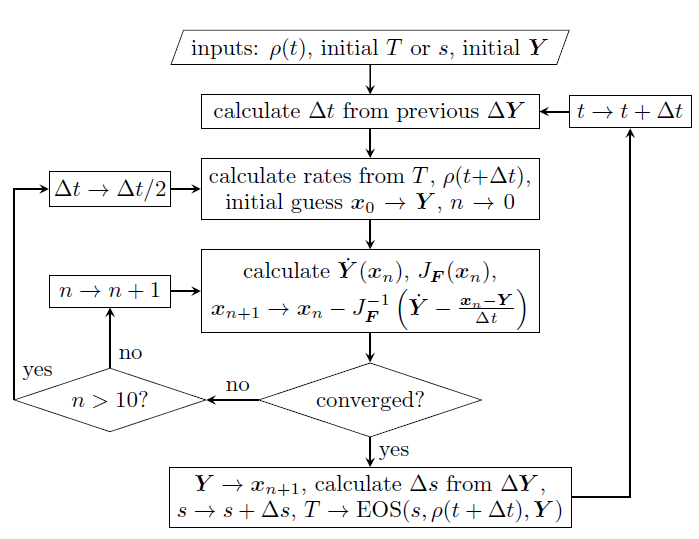
\includegraphics[width=0.7\linewidth]{22}}
	\caption{Упрощенный обзор адаптивного механизма временного шага, используемого в SkyNet. Если итерации NR не сходятся после 10 итераций, размер шага времени t сокращается в 2 раза, а шаг времени считается снова. Существуют и другие условия, которые может привести к неудачному шагу и последующей попытке с меньшим размером шага времени. Смотрите текст. После успешного шага времени следующий $\Delta t$ вычисляется из размера изменения обилий $\Delta Y$ (уравнение 2.58), и в этой точке $\Delta t$ может увеличиться или уменьшаться.}
	\label{ris:22}
\end{figure}

Очень редко необходимо перенормировать композицию. В этом случае каждое
обилие делится на общую массу, то есть,

$$(2.59)$$

и тогда новая композиция в точности удовлетворяет $...$. Хотя это искусственное впрыскивание или удаление энергии из системы, это полезно в крайнем случае, если временной шаг невелик, поскольку композиция далека от сохранения массы (но все же в пределах допуска погрешности). После перенормировки эволюция обычно выполняется нормально с большим временным шагом, чем раньше. Перенормируем, если временной шаг падает ниже определенного предела (обычно $10^{-16}$), или если было более 25 попыток увеличения размер шага, которые потерпели неудачу и  мы вынуждены сохранять размер шага постоянным. В таких случаях может быть, что временной шаг небольшой потому что критерий сходимости сохранения массы предотвращает временной шаг от увеличения. Если это так, то перенормировка обилия обычно помогает увеличить временной шаг, потому что после перенормировки сохранение массы в Уравнение (2.57) выполняется точно. Но в некоторых случаях, например, при попытке эволюциониовать сеть вблизи NSE с реакционными показателями, которые несовместимы с NSE (см. Раздел 2.6.1.1), временной шаг невелик, поскольку обилия изменяется быстро и поэтому перенормировка композиции не помогает.

\section{NSE evolution mode}
Если обилие приближается к композиции NSE, форвардная и обратная сильная ставки точно сбалансированы (раздел 2.2.3) (!!!the forward and inverse strong rates exactly balance). В этом случае все частные производные в Якобиане (уравнение 2.40) будет равен нулю, что приведет к сингулярному Якобиану. Однако Якобиан не является в точности сингулярным, поскольку слабые реакции (которые не находятся в равновесии со своими противоположностями) вносят ненулевые производные в якобиан. Тем не менее, по мере того, как сильные реакции переходят в равновесие, шаг времени становится очень малым, поскольку якобиан становится близким к численно сингулярному. Чтобы устранить эту проблему, SkyNet автоматически переключается с полной эволюции сети к схеме эволюции NSE, если масштаб временой шкалы сильной ядерной реакции становится короче шкалы времени, по которой изменяется плотность, и если температура выше некоторого порога (пользовательская настройка со значением по умолчанию 7 ГК). Полная сеть возвращается, когда эти условия больше не выполняются.

Если SkyNet определит, что переход на эволюцию NSE возможен, он вычисляет NSE из текущей внутренней энергии, плотности и электронной доли. Если энтропия и температура этой композиции NSE отличаются менее чем на $1\%$ (пользовательская настройка) от текущей энтропии и температуры сети, тогда он переключиться на NSE. В противном случае полная эволюция сети продолжится, и SkyNet будет пытаться пеерейти в режим эволюции NSE после следующего шага. Тест эволюции NSE режима, который демонстрирует его необходимость и согласованность, содержится в разделе 2.6.3.

В режиме эволюции NSE SkyNet больше не развивает обилие всех ядерных видов. Вместо этого SkyNet развивает энтропию $s$ и электронную долю $Y_e$ системы, которые может меняться из-за слабых реакций, таких как $\beta$-распад или взаимодействия нейтрино, которые могут изменять заряд нуклидов и нагревать материю. Напомним, что электронная доля равна $...$ и 
$$(2.60)$$
где $...$ задается уравнением (2.15) как функция от T,$\rho$ и Y. Температура задается EOS как функция от s,$\rho$ и Y. Y задается NSE как функция от s,$\rho$ и $Y_e$ (см. раздел 2.B.2). Таким образом, мы имеем

$$(2.61 - 64)$$

Скорость изменения энтропии получается из деления уравнения (2.50) на $\Delta t$,
а именно

$$(2.65)$$

Поскольку $...$, $...$ и $...$ известны, мы, таким образом, имеем два связанных ODE для $Y_e$ и s, которые SkyNet интегрирует с методом Рунге-Кутта-Фельберга 4 (5) (например, Burden et al., 2015, §5.5). Это метод четвертого порядка точности, который также оценивает ошибки 5-го порядка, которая используется для адаптивного управления интеграцией временного шага. Скорость нагрева можно рассчитать аналогично уравнению (2.55) как

$$(2.66)$$

Обратите внимание, что в режиме эволюции NSE мы развиваем только две переменные, и они меняются на аналогичных временных масштабах, потому что на них влияют слабые реакции. В этом однако, хотя слабые реакции охватывают большой диапазон временных масштабов, это не приводит к какой-либо жесткости, поскольку мы имеем дело только с суммой производных обилия в обоих уравнениях (2.60) и (2.65). Таким образом, мы можем безопасно использовать явный метод интеграции.

\end{document} 